%%% Ne pas modifier jusqu'à la ligne 25
\documentclass[a4paper,12pt]{book}
\usepackage[utf8]{inputenc}
\usepackage[french]{babel}
%%\usepackage{CJK}
\usepackage{yhmath}
\usepackage[left=2cm,right=2cm,top=3cm,bottom=2cm, headheight=1.5cm,headsep=1.5cm]{geometry}
%%\usepackage{CJKutf8}
\usepackage{amsfonts}
\usepackage{amsmath,amsfonts,amssymb,dsfont}
\usepackage{graphicx}
\usepackage{enumitem}		%\enumerate-resume
\usepackage[colorlinks=true,unicode={true},hyperindex=false, linkcolor=blue, urlcolor=blue]{hyperref}
\newcommand{\myref}[1]{\ref{#1} page \pageref{#1}}

\addto\captionsfrench{\def\tablename{Tableau}}  %légendes des tableaux
\renewcommand\thesection{\Roman{section}~-~} 
\renewcommand\thesubsection{\Roman{section}.\Alph{subsection}~-~} 
\renewcommand\thesubsubsection{\Roman{section}.\Alph{subsection}.\arabic{subsubsection}~-~} 

\newcommand{\conclusion}[1]{\newline \centerline{\fbox{#1}}}

\setcounter{secnumdepth}{3}
\parindent=0pt

\usepackage{fancyhdr}
\pagestyle{fancy}

\lhead{SJTU-ParisTech} 
%%%%%%%%%%%%%%%%%%%%%%%%%%%%%%%%%%
\chead{TR2}
\rhead{Daniel 518261910024}

\begin{document}
\renewcommand{\labelitemi}{$\blacktriangleright$}
\renewcommand{\labelitemii}{$\bullet$}


\section{calcul de la différence de marche}

\begin{figure}[h]
    \begin{center}
    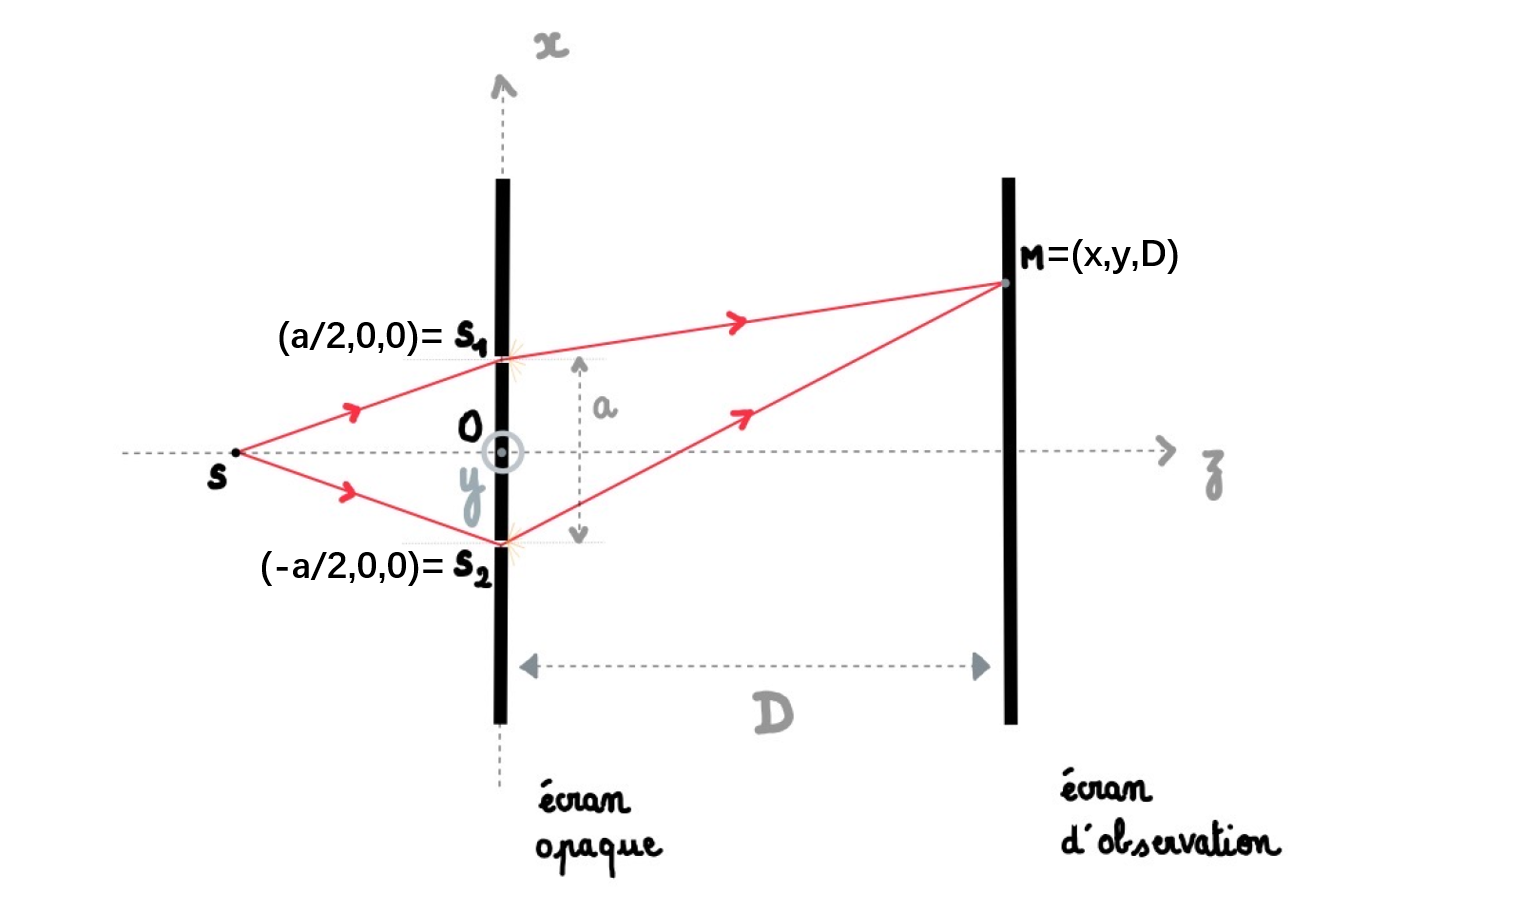
\includegraphics[scale=0.8]{tr2.png}
    \end{center}
    \caption{Expérience des trous de Young}
\end{figure}
On commence par $$\delta_{2/1}(M)=(SM)_2-(SM)_1$$
Supposons que l'expérience est fait dans un milieu homogène d'indice de fraction $n$: 
$(SM)_1=n*SM=n*S_1M+n*SS_1=(S_1M)+(SS_1)$, de même, $(SM)_2=(S_2M)+(SS_2)$, on arrive à 
$$\delta_{2/1}(M)=(SS_2)-(SS_1) + (S_2M)-(S_1M) $$
Car $S_1$ et $S_2$ sont symmétrique par rapport à l'axe $O_z$ sur lequelle $S$ se trouve, 
on a $SS_1=SS_2$, donc $(SS_1)=(SS_2)$, d'où
$$\delta_{2/1}(M)=(S_2M) - (S_1M)$$
On continue le calcul en supposant on fait l'expérience dans le vide: $n=1$. En appliquant les coordonnées, on a 
\begin{align*}
    \delta_{2/1}(M)&=S_2M - S_1M\\
                   &=\sqrt{\left(x+\frac{a}{2}\right)^2+(y+0)^2+(D+0)^2}-\sqrt{\left(x-\frac{a}{2}\right)^2+(y+0)^2+(D+0)^2}\\
                   &=D\left[\sqrt{1+\left(\frac{x+\frac{a}{2}}{D}\right)^2+(\frac{y}{D})^2}-\sqrt{1+\left(\frac{x-\frac{a}{2}}{D}\right)^2+(\frac{y}{D})^2}\right]
\end{align*} 
Lorsque l'on fait l'observation au voisinage de l'axe $O_z$, c'est à dire que $|x| \ll D, |y| \ll D$ et à grande distance $a \ll D$, 
on a $(x+\frac{a}{2}) \ll D$ et donc $\left(\frac{x+\frac{a}{2}}{D}\right)^2+(\frac{y}{D})^2 \ll 1$. Par développement limité à l'ordre 1 que 
$\sqrt{1+x} = 1+\frac{x}{2}$ lorsque $x\ll 1$, on a 
\begin{align*}
    \delta_{2/1}(M)&=D\left[\sqrt{1+\left(\frac{x+\frac{a}{2}}{D}\right)^2+(\frac{y}{D})^2}-\sqrt{1+\left(\frac{x-\frac{a}{2}}{D}\right)^2+(\frac{y}{D})^2}\right]\\
                   &=D\left[1+\frac{1}{2}\left(\frac{x+\frac{a}{2}}{D}\right)^2+\frac{1}{2}(\frac{y}{D})^2-\left(1+\frac{1}{2}\left(\frac{x-\frac{a}{2}}{D}\right)^2+\frac{1}{2}(\frac{y}{D})^2\right)\right]\\
\end{align*}
Finalement, on arrive à $\boxed{\delta_{2/1}(M)= \frac{ax}{D}}$ selon notre approximation. 
\end{document}